%Corps du document :
%\setlength{\parindent}{1cm}    

\section{Répartition des composants sur l'architecture n-tiers}

\subsection{Répartition des blocs applicatifs}

Les blocs \textbf{Produits}, \textbf{Client} et \textbf{Agence} seront implémentés sur le serveur du site central, mais également répliqués sur les serveurs des agences principales. L'architecture de ces données sera en \textbf{multi-maître}. Ainsi, chaque site pourra modifier les données. La gestion des conflits se fera si possible automatiquement, puis au besoin par l'intervention d'un responsable sur le site central.

Les blocs \textbf{Agence} et \textbf{Client}, en plus d'être répliqués, seront répartis. La base de données de chaque agence contiendra seulement les informations des sous-agences qu'elle gère.

Même si les modifications de \textbf{Client} sont nombreuses, peu de conflict seront générés car peu de modifications seront émises à partir du site central. L'intérêt de cette réplication est la sauvegarde des données du client, et un accès aux données accéléré.

Les blocs \textbf{Agenda} et \textbf{Contact} seront répartis. Aucune information ne sera sur le site central. Chaque agence principale gèrera ces propres informations.

\begin {center}
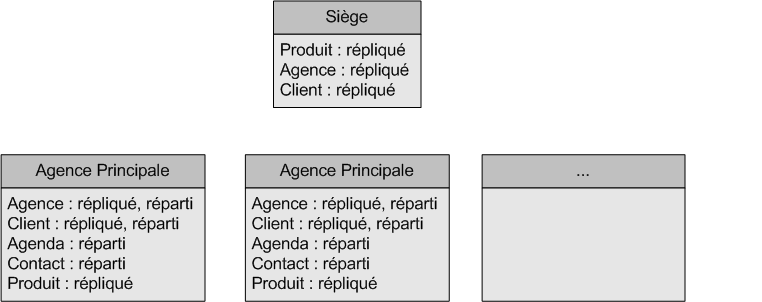
\includegraphics[width=\textwidth]{repartition_bloc.png}
\end {center}

\subsection{Principaux flux applicatifs échangés}

\begin{itemize}
\item Ajout de nouvelles données
\item Consultation des données
\item Mise à jour des données
\item Sauvegarde des données
\item Réplication des données
\end{itemize}
